\subsection{Comparación de los cuatro modelos por clase}

La Tabla~\ref{tab:modelos4} reporta las métricas de los cuatro modelos base en el conjunto de prueba, cada uno con su propio umbral (el que maximiza el F1 de la clase 1 por validación cruzada en el entrenamiento). Los conteos de las matrices de confusión y las curvas ROC y de precisión--sensibilidad están en el Anexo~H. El mayor PR-AUC correspondió a Random Forest (0.411), el mayor ROC-AUC a Random Forest (0.680), la mayor sensibilidad a XGBoost (0.819) y el mayor F1 a Random Forest (0.459).

La diferencia de PR-AUC entre Random Forest y Regresión logística es de 0.020; es pequeña, por lo que la elección de Random Forest debe leerse como una preferencia débil y no como una superioridad clara.

\begin{table}[H]
  \caption{Métricas de los cuatro modelos base en el conjunto de prueba, con el umbral de cada modelo (F1 máximo por validación cruzada en entrenamiento).}
  \label{tab:modelos4}
  \tablabase\scriptsize
  \begin{tabular}{|l|c|c|c|c|c|c|c|c|}
    \hline
    \enc{Modelo} & \enc{PR-AUC} & \enc{ROC-AUC} & \enc{Umbral} & \enc{Sens.} & \enc{Espec.} & \enc{Prec.} & \enc{F1} & \enc{Ex. bal.} \\ \hline
    Regresión logística & 0.391 & 0.667 & 0.470 & 0.673 & 0.574 & 0.341 & 0.453 & 0.624 \\ \hline
    Árbol de decisión & 0.263 & 0.536 & 0.050 & 0.300 & 0.773 & 0.302 & 0.301 & 0.536 \\ \hline
    Random Forest & 0.411 & 0.680 & 0.230 & 0.735 & 0.521 & 0.334 & 0.459 & 0.628 \\ \hline
    XGBoost & 0.368 & 0.648 & 0.240 & 0.819 & 0.359 & 0.295 & 0.434 & 0.589 \\ \hline
  \end{tabular}
\end{table}




\subsection{Sensibilidad al umbral de decisión}

La Figura~\ref{fig:umbral} muestra cómo cambian las métricas del modelo final al variar el umbral. Con 0.30 la sensibilidad sube a 0.959, pero la precisión baja a 0.261 y el modelo genera 3355 alertas sobre 3699 registros; con 0.42 (umbral adoptado) la sensibilidad es 0.693, la precisión 0.335 y las alertas 1887; con 0.60 la sensibilidad cae a 0.106 y la precisión sube a 0.524. No existe un umbral que alcance a la vez sensibilidad y precisión altas: la elección refleja una decisión sobre qué error se tolera más. Los valores para otros umbrales están en el Anexo~H.

\begin{figure}[H]
  \centering
  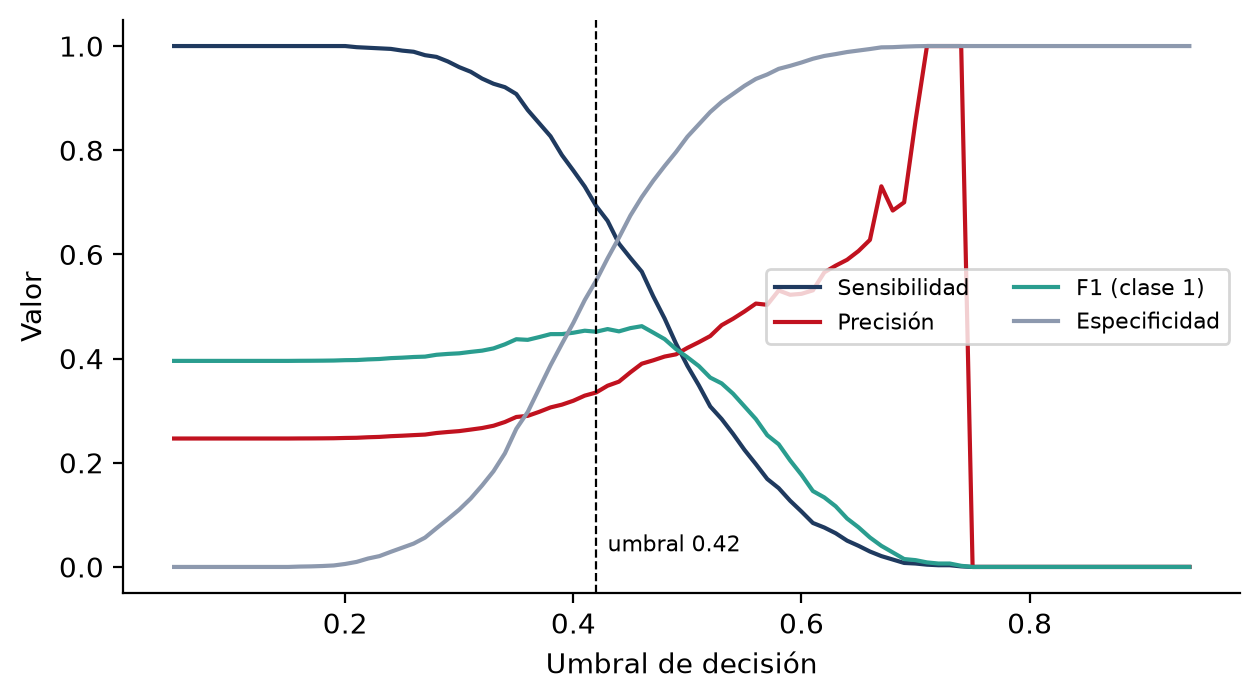
\includegraphics[width=0.75\textwidth]{figuras/anexo-umbral.png}
  \caption{Métricas del modelo final según el umbral de decisión (conjunto de prueba). Elaboración propia.}
  \label{fig:umbral}
\end{figure}



\subsection{Calibración de las probabilidades}

La calibración indica si una probabilidad predicha corresponde a la frecuencia real de casos \cite{steyerberg2019clinical}. El error de Brier del modelo final es 0.205, frente a 0.186 de un predictor que solo usa la prevalencia, es decir, es peor: las probabilidades del modelo no están calibradas. La probabilidad media predicha es 0.427 y la prevalencia observada es 0.247. En el decil más bajo la probabilidad media es 0.264 y la proporción observada 0.105; en el más alto, 0.608 y 0.505.

La probabilidad media supera la prevalencia porque el modelo se entrenó con ponderación de clases; por eso las probabilidades no deben leerse como riesgo absoluto, sino como una puntuación para ordenar casos. Esta es otra razón para no interpretar los niveles de riesgo (BAJO, MEDIO, ALTO) de la API como probabilidades reales. La curva y la distribución de probabilidades están en el Anexo~H (Figura~\ref{fig:calibracion}).



\subsection{Desempeño por subgrupos}

La Figura~\ref{fig:subgrupos} muestra la sensibilidad del modelo final (umbral 0.42) en subgrupos del conjunto de prueba nacional, con intervalos de Wilson. En el conjunto nacional, según el área, la sensibilidad va de 0.525 (Urbano; 480 casos) a 0.880 (Rural; 432 casos); según el sexo, la sensibilidad va de 0.659 (Mujer; 402 casos) a 0.720 (Hombre; 510 casos); según el grupo de edad, la sensibilidad va de 0.505 (36-59; 295 casos) a 0.892 (12-23; 259 casos).

Las diferencias son marcadas: entre Urbano y Rural los intervalos no se traslapan, y la prevalencia muestral es de 21.4\,\% y 29.7\,\% respectivamente; entre 36-59 y 12-23 los intervalos no se traslapan, y la prevalencia muestral es de 19.3\,\% y 34.0\,\% respectivamente. Con un umbral único, el modelo identifica una proporción mayor de los casos donde la prevalencia es mayor y una proporción menor donde es menor. Por eso la sensibilidad global (0.693) oculta diferencias importantes: en los subgrupos con menor prevalencia se omite cerca de la mitad de los casos. Un uso aplicado exigiría revisar el umbral por grupo. En el sexo la diferencia es menor.

El detalle, con especificidad y ROC-AUC, y los subgrupos de Tungurahua (muy pequeños, por lo que solo son indicativos) están en el Anexo~H.

\begin{figure}[H]
  \centering
  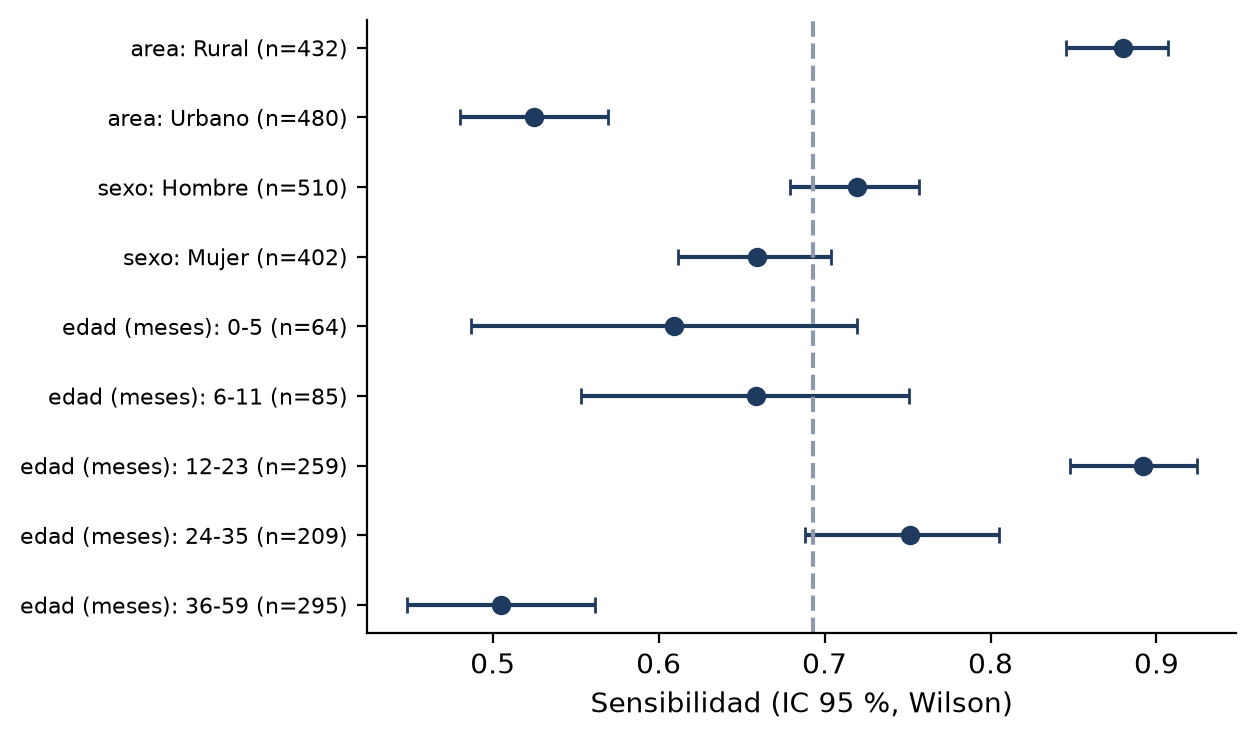
\includegraphics[width=0.8\textwidth]{figuras/anexo-subgrupos.png}
  \caption{Sensibilidad del modelo final por subgrupos en la prueba nacional (línea punteada: sensibilidad global). Elaboración propia.}
  \label{fig:subgrupos}
\end{figure}



\subsection{Análisis de errores}

La Figura~\ref{fig:errores} descompone las clasificaciones por grupo de edad. La proporción de casos omitidos (falsos negativos entre los casos reales) fue mayor en el grupo de 36-59 meses (49.5\,\%) y menor en el de 12-23 meses (10.8\,\%). La proporción de falsas alarmas (falsos positivos entre los no casos) fue mayor en 12-23 meses (75.3\,\%) y menor en 36-59 meses (29.1\,\%). Como la edad es la variable con mayor importancia del modelo, es esperable que los errores dependan de ella; un uso aplicado exigiría revisar el desempeño por edad antes de fijar un umbral único.

\begin{figure}[H]
  \centering
  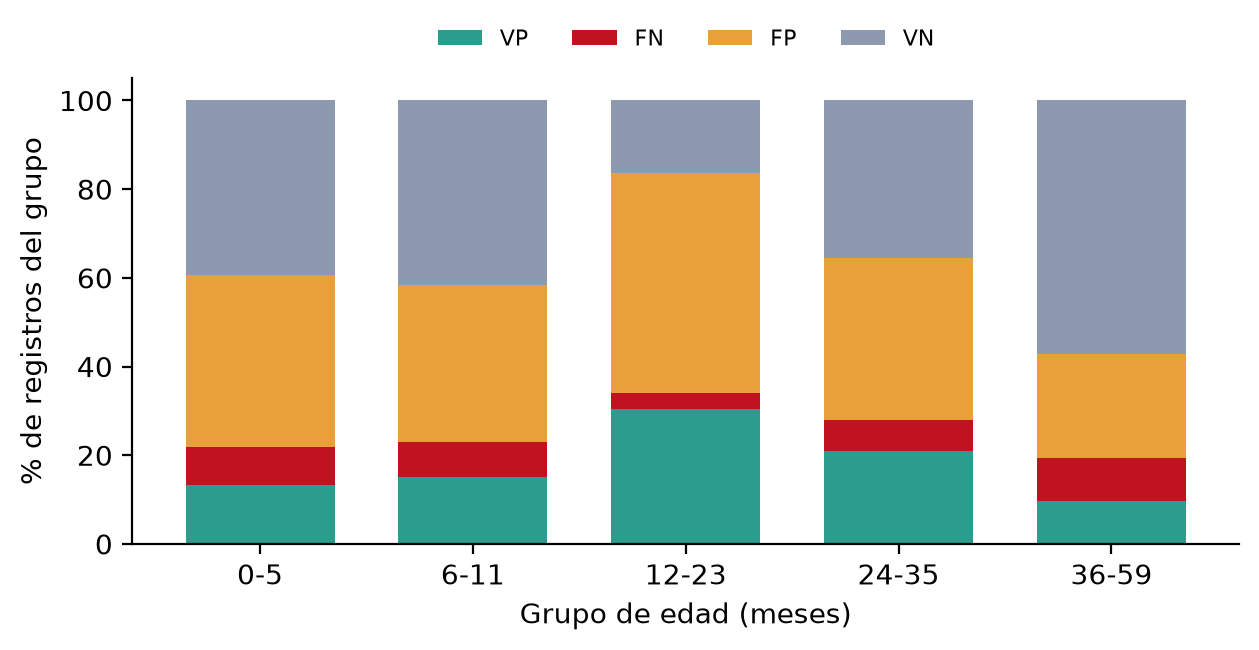
\includegraphics[width=0.75\textwidth]{figuras/anexo-errores-edad.png}
  \caption{Composición de las clasificaciones por grupo de edad (umbral 0.42). VP: verdaderos positivos; FN: falsos negativos; FP: falsos positivos; VN: verdaderos negativos. Elaboración propia.}
  \label{fig:errores}
\end{figure}



\subsection{Prueba sin las variables de diseño muestral}

Como \texttt{factor\_expansion} y \texttt{estrato} no describen al niño, se entrenó un Random Forest con los mismos hiperparámetros y la misma partición, pero sin esas dos variables. La Tabla~\ref{tab:sindiseno} muestra el resultado: el ROC-AUC pasa de 0.677 a 0.679 (diferencia de +0.002) y el PR-AUC de 0.409 a 0.408 (diferencia de -0.001). La diferencia es pequeña, por lo que el desempeño no depende de forma importante de esas dos variables y el modelo sin ellas es una alternativa más limpia. Con el umbral propio de esta versión (0.40, elegido por validación cruzada en el entrenamiento) la sensibilidad es 0.777 y la precisión 0.319. Esta prueba es un análisis de sensibilidad complementario: el modelo evaluado y desplegado sigue siendo el de 114 variables.

\begin{table}[H]
  \caption{Comparación del modelo final con una versión sin las variables de diseño muestral.}
  \label{tab:sindiseno}
  \tablabase\scriptsize
  \begin{tabular}{|p{5.6cm}|c|c|c|c|c|c|}
    \hline
    \enc{Modelo} & \enc{ROC-AUC} & \enc{PR-AUC} & \enc{Sens.} & \enc{Espec.} & \enc{Prec.} & \enc{Ex. bal.} \\ \hline
    Modelo final (con 114 variables), umbral 0.42 & 0.677 & 0.409 & 0.693 & 0.550 & 0.335 & 0.621 \\ \hline
    Sin \texttt{factor\_expansion} ni \texttt{estrato} (112 variables), umbral 0.42 & 0.679 & 0.408 & 0.717 & 0.540 & 0.338 & 0.629 \\ \hline
    Sin variables de diseño, umbral propio 0.40 & 0.679 & 0.408 & 0.777 & 0.456 & 0.319 & 0.617 \\ \hline
  \end{tabular}
\end{table}



